% vim: set ts=4 sw=4 tw=80 noexpandtab:

\documentclass{42-en}

%******************************************************************************%
%                                                                              %
%                                   Prologue                                   %
%                                                                              %
%******************************************************************************%
\usepackage[
    type={CC},
    modifier={by-nc-sa},
    version={4.0},
]{doclicense}

%****************************************************************%
%                  Re/definition of commands                     %
%****************************************************************%

\newcommand{\ailogo}[1]{\def \@ailogo {#1}}\ailogo{assets/42ai_logo.pdf}

%%  Redefine \maketitle
\makeatletter
\def \maketitle {
  \begin{titlepage}
    \begin{center}
	%\begin{figure}[t]
	  %\includegraphics[height=8cm]{\@ailogo}
	  
\includegraphics[height=8cm]{assets/42ai_logo.pdf}
	%\end{figure}
      \vskip 5em
      {\huge \@title}
      \vskip 2em
      {\LARGE \@subtitle}
      \vskip 4em
    \end{center}
    %\begin{center}
	  %\@author
    %\end{center}
	%\vskip 5em
  \vfill
  \begin{center}
    \emph{\summarytitle : \@summary}
  \end{center}
  \vspace{2cm}
  %\vskip 5em
  %\doclicenseThis
  \end{titlepage}
}
\makeatother

\makeatletter
\def \makeheaderfilesforbidden
{
  \noindent
  \begin{tabularx}{\textwidth}{|X X  X X|}
    \hline
  \multicolumn{1}{|>{\raggedright}m{1cm}|}
  {\vskip 2mm 
\includegraphics[height=1cm]{assets/42ai_logo.pdf}} &
  \multicolumn{2}{>{\centering}m{12cm}}{\small Exercise : \@exnumber } &
  \multicolumn{1}{ >{\raggedleft}p{1.5cm}|}
%%              {\scriptsize points : \@exscore} \\ \hline
              {} \\ \hline

  \multicolumn{4}{|>{\centering}m{15cm}|}
              {\small \@extitle} \\ \hline

  \multicolumn{4}{|>{\raggedright}m{15cm}|}
              {\small Turn-in directory : \ttfamily
                $ex\@exnumber/$ }
              \\ \hline
  \multicolumn{4}{|>{\raggedright}m{15cm}|}
              {\small Files to turn in : \ttfamily \@exfiles }
              \\ \hline

  \multicolumn{4}{|>{\raggedright}m{15cm}|}
              {\small Forbidden functions : \ttfamily \@exforbidden }
              \\ \hline

%%  \multicolumn{4}{|>{\raggedright}m{15cm}|}
%%              {\small Remarks : \ttfamily \@exnotes }
%%              \\ \hline
\end{tabularx}
%% \exnotes
\exrules
\exmake
\exauthorize{None}
\exforbidden{None}
\extitle{}
\exnumber{}
}
\makeatother

%%  Syntactic highlights
\makeatletter
\newenvironment{pythoncode}{%
  \VerbatimEnvironment
  \usemintedstyle{emacs}
  \minted@resetoptions
  \setkeys{minted@opt}{bgcolor=black,formatcom=\color{lightgrey},fontsize=\scriptsize}
  \begin{figure}[ht!]
    \centering
    \begin{minipage}{16cm}
      \begin{VerbatimOut}{\jobname.pyg}}
{%[
      \end{VerbatimOut}
      \minted@pygmentize{c}
      \DeleteFile{\jobname.pyg}
    \end{minipage}
\end{figure}}
\makeatother

\usemintedstyle{native}

\begin{document}

% =============================================================================%
%                     =====================================                    %

\title{Python \& ML - Module 03}
\subtitle{Numpy}
\author{
  Maxime Choulika (cmaxime), Pierre Peigné (ppeigne), Matthieu David (mdavid)
}

\summary
{
	Today you will learn how to use the Python library that will allow you to manipulate
  multidimensional arrays (vectors) and perform complex mathematical operations on them.
}

\maketitle
%******************************************************************************%
%                                                                              %
%                        Common Instructions                                   %
%                          for Python Projects                                 %
%                                                                              %
%******************************************************************************%

\chapter{Common Instructions}
\begin{itemize}
  \item The version of Python recommended to use is 3.7, you can
  check the version of Python with the following command: \texttt{python -V}
  
  \item The norm: during this piscine, it is recommended to follow the
  \href{https://www.python.org/dev/peps/pep-0008/}{PEP 8 standards}, though it is not mandatory.
  You can install \href{https://pypi.org/project/pycodestyle}{pycodestyle} which
  is a tool to check your Python code.
  
  \item The function \texttt{eval} is never allowed.
  
  \item The exercises are ordered from the easiest to the hardest.
  
  \item Your exercises are going to be evaluated by someone else,
  so make sure that your variable names and function names are appropriate and civil. 
  
  \item Your manual is the internet.
  
  \item You can also ask questions in the \texttt{\#bootcamps} channel in the \href{https://42-ai.slack.com}{42AI}
  or \href{42born2code.slack.com}{42born2code}.
  
  \item If you find any issue or mistakes in the subject please create an issue on \href{https://github.com/42-AI/bootcamp_python/issues}{42AI repository on Github}.  
  
  \item We encourage you to create test programs for your
  project even though this work \textbf{won't have to be
  submitted and won't be graded}. It will give you a chance
  to easily test your work and your peers’ work. You will find
  those tests especially useful during your defence. Indeed,
  during defence, you are free to use your tests and/or the
  tests of the peer you are evaluating.
  
  \item Submit your work to your assigned git repository. Only the work in the
  git repository will be graded. If Deepthought is assigned to grade your
  work, it will be run after your peer-evaluations.
  If an error happens in any section of your work during Deepthought's grading,
  the evaluation will stop.
\end{itemize}
\newpage
\tableofcontents
\startexercices

%                     =====================================                    %
% =============================================================================%


%******************************************************************************%
%                                                                              %
%                                   Exercises                                  %
%                                                                              %
%******************************************************************************%

% ============================================== %
% ===========================(start ex 00)       %
\chapter{Exercise 00}
\extitle{NumPyCreator}
\turnindir{ex00}
\exnumber{00}
\exfiles{NumPyCreator.py}
\exforbidden{None}
\makeheaderfilesforbidden

% ================================== %
\section*{Objective}
% ---------------------------------- %
Introduction to Numpy library.

% ================================== %
\section*{Instructions}
% ---------------------------------- %
Write a class named \texttt{NumPyCreator}, that implements all of the following methods.
Each method receives as an argument a different type of data structure and transforms it into a Numpy array:
\begin{itemize}
  \item \texttt{from\_list(self, lst)}: takes a list or nested lists and returns its corresponding Numpy array.
  \item \texttt{from\_tuple(self, tpl)}: takes a tuple or nested tuples and returns its corresponding Numpy array.
  \item \texttt{from\_iterable(self, itr)}: takes an iterable and returns an array which contains all its elements.
  \item \texttt{from\_shape(self, shape, value)}: returns an array filled with the same value.
  The first argument is a tuple which specifies the shape of the array, and the second argument specifies the value of the elements. 
  This value must be 0 by default.
  \item \texttt{random(self, shape)}: returns an array filled with random values.
  It takes as an argument a tuple which specifies the shape of the array.
  \item \texttt{identity(self, n)}: returns an array representing the identity matrix of size n.
\end{itemize}


\textit{\textbf{BONUS:}} Add to those methods an optional argument which specifies the datatype (dtype) of the array (e.g. to represent its elements as integers, floats, ...)

\hint All those methods can be implemented in one line. You only need to find the right Numpy functions.

% ================================== %
\section*{Examples}
% ---------------------------------- %
\begin{minted}[bgcolor=darcula-back,formatcom=\color{lightgrey},fontsize=\scriptsize]{python}
from NumpyCreator import NumpyCreator
npc = NumpyCreator()

npc.from_list([[1,2,3],[6,3,4]])
# Output :
array([[1, 2, 3],
       [6, 3, 4]])


npc.from_list([[1,2,3],[6,4]])
# Output :
None


npc.from_list([[1,2,3],['a','b','c'],[6,4,7]])
# Output :
array([['1','2','3'],
       ['a','b','c'],
       ['6','4','7'], dtype='<U21'])


npc.from_list(((1,2),(3,4)))
# Output :
None


npc.from_tuple(("a", "b", "c"))
# Output :
array(['a', 'b', 'c'])


npc.from_tuple(["a", "b", "c"])
# Output :
None


npc.from_iterable(range(5))
# Output :
array([0, 1, 2, 3, 4])


shape=(3,5)
npc.from_shape(shape)
# Output :
array([[0, 0, 0, 0, 0],
       [0, 0, 0, 0, 0],
       [0, 0, 0, 0, 0]])


npc.random(shape)
# Output :
array([[0.57055863, 0.23519999, 0.56209311, 0.79231567, 0.213768 ],
      [0.39608366, 0.18632147, 0.80054602, 0.44905766, 0.81313615],
      [0.79585328, 0.00660962, 0.92910958, 0.9905421 , 0.05244791]])


npc.identity(4)
# Output :
array([[1., 0., 0., 0.],
       [0., 1., 0., 0.],
       [0., 0., 1., 0.],
       [0., 0., 0., 1.]])
\end{minted}

% ===========================(fin ex 00)         %
% ============================================== %
\newpage

% ============================================== %
% ===========================(start ex 01)       %
\chapter{Exercise 01}
\extitle{ImageProcessor}
\turnindir{ex01}
\exnumber{01}
\exfiles{ImageProcessor.py}
\exforbidden{None}
\makeheaderfilesforbidden


% ================================= %
\section*{Objective}
% --------------------------------- %
Basic manipulation of image via matplotlib library.


% ================================= %
\section*{Instructions}
% --------------------------------- %
Build a tool that will be helpful to load and display images in the upcoming exercises.

Write a class named \texttt{ImageProcessor} that implements the following methods:
\begin{itemize}
  \item \texttt{load(path)}: opens the PNG file specified by the \texttt{path} argument and returns an array with the RGB values of the pixels image. It must display a message specifying the dimensions of the image (e.g. 340 x 500).

  \item \texttt{display(array)}: takes a numpy array as an argument and displays the corresponding RGB image.
\end{itemize}

You must handle errors, if the file passed as argument does not exist or if it can't be read as an image, with an appropriate message of your choice.

\hint{You can use the library of your choice for this exercise,
but converting the image to a numpy array is mandatory.
The goal of this exercise is to dispense with the technicality of loading and displaying images,
so that you can focus on array manipulation in the upcoming exercises.
}

% ================================= %
\section*{Examples}
% --------------------------------- %
\begin{minted}[bgcolor=darcula-back,formatcom=\color{lightgrey},fontsize=\scriptsize]{python}
from ImageProcessor import ImageProcessor
imp = ImageProcessor()
arr = imp.load("non_existing_file.png")
# Output :
Exception: FileNotFoundError -- strerror: No such file or directory


print(arr)
# Output :
None


arr = imp.load("empty_file.png")
# Output :
Exception: OSError -- strerror: None


print(arr)
# Output :
None


arr = imp.load("../resources/42AI.png")
# Output :
Loading image of dimensions 200 x 200


arr
# Output :
array([[[0.03529412, 0.12156863, 0.3137255 ],
        [0.03921569, 0.1254902 , 0.31764707],
        [0.04313726, 0.12941177, 0.3254902 ],
        ...,
        [0.02745098, 0.07450981, 0.22745098],
        [0.02745098, 0.07450981, 0.22745098],
        [0.02352941, 0.07058824, 0.22352941]],

       [[0.03921569, 0.11764706, 0.30588236],
        [0.03529412, 0.11764706, 0.30980393],
        [0.03921569, 0.12156863, 0.30980393],
        ...,
        [0.02352941, 0.07450981, 0.22745098],
        [0.02352941, 0.07450981, 0.22745098],
        [0.02352941, 0.07450981, 0.22745098]],

       [[0.03137255, 0.10980392, 0.2901961 ],
        [0.03137255, 0.11372549, 0.29803923],
        [0.03529412, 0.11764706, 0.30588236],
        ...,
        [0.02745098, 0.07450981, 0.23137255],
        [0.02352941, 0.07450981, 0.22745098],
        [0.02352941, 0.07450981, 0.22745098]],

       ...,

       [[0.03137255, 0.07450981, 0.21960784],
        [0.03137255, 0.07058824, 0.21568628],
        [0.03137255, 0.07058824, 0.21960784],
        ...,
        [0.03921569, 0.10980392, 0.2784314 ],
        [0.03921569, 0.10980392, 0.27450982],
        [0.03921569, 0.10980392, 0.27450982]],

       [[0.03137255, 0.07058824, 0.21960784],
        [0.03137255, 0.07058824, 0.21568628],
        [0.03137255, 0.07058824, 0.21568628],
        ...,
        [0.03921569, 0.10588235, 0.27058825],
        [0.03921569, 0.10588235, 0.27058825],
        [0.03921569, 0.10588235, 0.27058825]],

       [[0.03137255, 0.07058824, 0.21960784],
        [0.03137255, 0.07058824, 0.21176471],
        [0.03137255, 0.07058824, 0.21568628],
        ...,
        [0.03921569, 0.10588235, 0.26666668],
        [0.03921569, 0.10588235, 0.26666668],
        [0.03921569, 0.10588235, 0.26666668]]], dtype=float32)


imp.display(arr)
\end{minted}

\begin{figure}[h!]
  \centering
  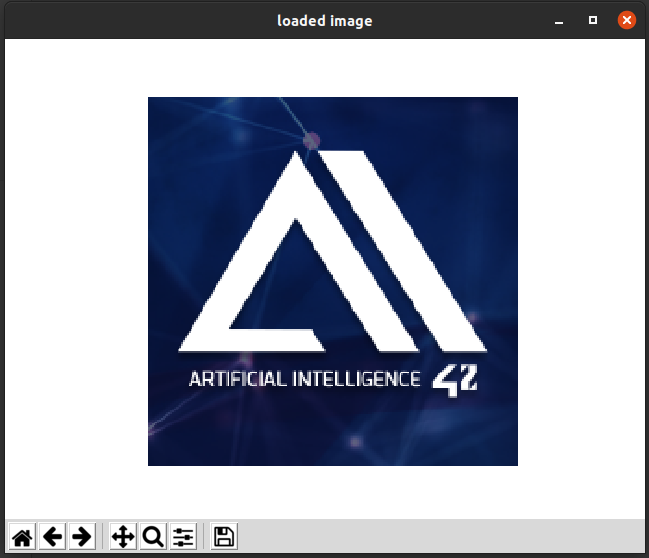
\includegraphics[scale=0.5]{assets/capture_display_img.png}
\end{figure}

The image must to be displayed in a separate window when running in the console.

% ===========================(fin ex 01)         %
% ============================================== %

\newpage

% ============================================== %
% ===========================(start ex 02)       %
\chapter{Exercise 02}
\extitle{ScrapBooker}
\turnindir{ex02}
\exnumber{02}
\exfiles{ScrapBooker.py}
\exforbidden{None}
\makeheaderfilesforbidden

% ================================= %
\section*{Objective}
% --------------------------------- %
Manipulation and initiation to slicing method on numpy arrays.

% ================================= %
\section*{Instructions}
% --------------------------------- %
Implement a class named \texttt{ScrapBooker} with the following methods:
\begin{itemize}
  \item \texttt{crop},
  \item \texttt{thin},
  \item \texttt{juxtapose},
  \item \texttt{mosaic}.
\end{itemize}

\begin{minted}[bgcolor=darcula-back,formatcom=\color{lightgrey},fontsize=\scriptsize]{python}
# within the class
def crop(self, array, dim, position=(0,0)):
    """
    Crops the image as a rectangle via dim arguments (being the new height
    and width of the image) from the coordinates given by position arguments.
    Args:
    -----
      array: numpy.ndarray
      dim: tuple of 2 integers.
      position: tuple of 2 integers.
    Return:
    -------
      new_arr: the cropped numpy.ndarray.
      None (if combinaison of parameters not compatible).
    Raise:
    ------
      This function should not raise any Exception.
    """
    ... your code ...

def thin(self, array, n, axis):
    """
    Deletes every n-th line pixels along the specified axis (0: vertical, 1: horizontal)
    Args:
    -----
      array: numpy.ndarray.
      n: non null positive integer lower than the number of row/column of the array
         (depending of axis value).
      axis: positive non null integer.
    Return:
    -------
      new_arr: thined numpy.ndarray.
      None (if combinaison of parameters not compatible).
    Raise:
    ------
      This function should not raise any Exception.
    """
    ... your code ...

def juxtapose(self, array, n, axis):
    """
    Juxtaposes n copies of the image along the specified axis.
    Args:
    -----
      array: numpy.ndarray.
      n: positive non null integer.
      axis: integer of value 0 or 1.
    Return:
    -------
      new_arr: juxtaposed numpy.ndarray.
      None (combinaison of parameters not compatible).
    Raises:
    -------
      This function should not raise any Exception.
    """
    ... your code ...

def mosaic(self, array, dim):
    """
    Makes a grid with multiple copies of the array. The dim argument specifies
    the number of repetition along each dimensions.
    Args:
    -----
      array: numpy.ndarray.
      dim: tuple of 2 integers.
    Return:
    -------
      new_arr: mosaic numpy.ndarray.
      None (combinaison of parameters not compatible).
    Raises:
    -------
      This function should not raise any Exception.
      """
      ... your code ...
\end{minted}


In this exercise, when specifying positions or dimensions, we will assume
that the first coordinate is counted along the vertical axis starting from
the top, and that the second coordinate is counted along the horizontal axis
starting from the left. Indexing starts from 0.

\parbox{\textwidth}{
  e.g.:\\
  (1,3)\\
  .....\\
  ...x.\\
  .....}


% ================================= %
\section*{Examples}
% --------------------------------- %
\begin{minted}[bgcolor=darcula-back,formatcom=\color{lightgrey},fontsize=\scriptsize]{python}
import numpy as np
from ScrapBooker import ScrapBooker

spb = ScrapBooker()
arr1 = np.arange(0,25).reshape(5,5)
spb.crop(arr1, (3,1),(1,0))
#Output :
array([[ 5],
       [10],
       [15]])


arr2 = np.array("A B C D E F G H I".split() * 6).reshape(-1,9)
spb.thin(arr2,3,0)
#Output :
array([['A', 'B', 'D', 'E', 'G', 'H', 'J', 'K'],
       ['A', 'B', 'D', 'E', 'G', 'H', 'J', 'K'],
       ['A', 'B', 'D', 'E', 'G', 'H', 'J', 'K'],
       ['A', 'B', 'D', 'E', 'G', 'H', 'J', 'K'],
       ['A', 'B', 'D', 'E', 'G', 'H', 'J', 'K'],
       ['A', 'B', 'D', 'E', 'G', 'H', 'J', 'K']], dtype='<U1')


arr3 = np.array([[1, 2, 3],[1, 2, 3],[1, 2, 3]])
spb.juxtapose(arr3, 3, 1)
#Output :
array([[1, 2, 3, 1, 2, 3, 1, 2, 3],
       [1, 2, 3, 1, 2, 3, 1, 2, 3],
       [1, 2, 3, 1, 2, 3, 1, 2, 3]])
\end{minted}

% ===========================(fin ex 02)         %
% ============================================== %

\newpage

% ============================================== %
% ===========================(start ex 03)       %
\chapter{Exercise 03}
\extitle{ColorFilter}
\turnindir{ex03}
\exnumber{03}
\exfiles{ColorFilter.py}
\exforbidden{None}
\makeheaderfilesforbidden


% ================================= %
\section*{Objective}
% --------------------------------- %
Manipulation of loaded image via numpy arrays, broadcasting.


% ================================= %
\section*{Instructions}
% --------------------------------- %
You have to develop a tool that can apply a variety of color filters on images.
For this exercise, the authorized functions and operators are specified for each methods.
You are not allowed to use anything else.

Write a class named \texttt{ColorFilter} with 6 methods with the following exact signatures:

\begin{minted}[bgcolor=darcula-back,formatcom=\color{lightgrey},fontsize=\scriptsize]{python}
def invert(self, array):
    """
    Inverts the color of the image received as a numpy array.
    Args:
    -----
        array: numpy.ndarray corresponding to the image.
    Return:
    -------
        array: numpy.ndarray corresponding to the transformed image.
        None: otherwise.
    Raises:
    -------
        This function should not raise any Exception.
    """
\end{minted}
\begin{minted}[bgcolor=darcula-back,formatcom=\color{lightgrey},fontsize=\scriptsize]{python}
def to_blue(self, array):
    """
    Applies a blue filter to the image received as a numpy array.
    Args:
    -----
        array: numpy.ndarray corresponding to the image.
    Return:
    -------
        array: numpy.ndarray corresponding to the transformed image.
        None: otherwise.
    Raises:
    -------
        This function should not raise any Exception.
    """
\end{minted}
\begin{minted}[bgcolor=darcula-back,formatcom=\color{lightgrey},fontsize=\scriptsize]{python}
def to_green(self, array):
    """
    Applies a green filter to the image received as a numpy array.
    Args:
    -----
        array: numpy.ndarray corresponding to the image.
    Return:
    -------
        array: numpy.ndarray corresponding to the transformed image.
        None: otherwise.
    Raises:
    -------
        This function should not raise any Exception.
    """
\end{minted}
\begin{minted}[bgcolor=darcula-back,formatcom=\color{lightgrey},fontsize=\scriptsize]{python}
def to_red(self, array):
    """
    Applies a red filter to the image received as a numpy array.
    Args:
    -----
        array: numpy.ndarray corresponding to the image.
    Return:
    -------
        array: numpy.ndarray corresponding to the transformed image.
        None: otherwise.
    Raises:
    -------
        This function should not raise any Exception.
    """
\end{minted}
\begin{minted}[bgcolor=darcula-back,formatcom=\color{lightgrey},fontsize=\scriptsize]{python}
def to_celluloid(self, array):
    """
    Applies a celluloid filter to the image received as a numpy array.
    Celluloid filter must display at least four thresholds of shades.
    Be careful! You are not asked to apply black contour on the object,
    you only have to work on the shades of your images.
    Remarks:
        celluloid filter is also known as cel-shading or toon-shading.
    Args:
    -----
        array: numpy.ndarray corresponding to the image.
    Return:
    -------
        array: numpy.ndarray corresponding to the transformed image.
        None: otherwise.
    Raises:
    -------
        This function should not raise any Exception.
    """
\end{minted}
\begin{minted}[bgcolor=darcula-back,formatcom=\color{lightgrey},fontsize=\scriptsize]{python}
def to_grayscale(self, array, filter, **kwargs):
    """
    Applies a grayscale filter to the image received as a numpy array.
    For filter = 'mean'/'m': performs the mean of RBG channels.
    For filter = 'weight'/'w': performs a weighted mean of RBG channels.
    Args:
    -----
        array: numpy.ndarray corresponding to the image.
        filter: string with accepted values in ['m','mean','w','weight']
        weights: [kwargs] list of 3 floats where the sum equals to 1,
                 corresponding to the weights of each RBG channels.
    Return:
    -------
        array: numpy.ndarray corresponding to the transformed image.
        None: otherwise.
    Raises:
    -------
        This function should not raise any Exception.
    """
\end{minted}

You have some restrictions on the authorized methods and operators
for each filter method in class \texttt{ColorFilter}:
\begin{itemize}
  \item \texttt{invert}:
  \begin{itemize}
    \item Authorized functions: \texttt{.copy}.
    \item Authorized operators: \texttt{+},\texttt{-},\texttt{=}.
  \end{itemize}
  \item \texttt{to\_blue}:
  \begin{itemize}
    \item Authorized functions: \texttt{.copy}, \texttt{.zeros},\texttt{.shape},\texttt{.dstack}.
    \item Authorized operators: \texttt{=}.
  \end{itemize}
  \item \texttt{to\_green}:
  \begin{itemize}
    \item Authorized functions: \texttt{.copy}.
    \item Authorized operators: \texttt{*}, \texttt{=}.
  \end{itemize}
  \item \texttt{to\_red}:
  \begin{itemize}
    \item Authorized functions: \texttt{.copy}, \texttt{.to\_green},\texttt{.to\_blue}.
    \item Authorized operators: \texttt{-},\texttt{+}, \texttt{=}.
  \end{itemize}
  \item \texttt{to\_celluloid(array)}:
  \begin{itemize}
    \item Authorized functions: \texttt{.copy}, \texttt{.arange},\texttt{.linspace}, \texttt{.min}, \texttt{.max}.
    \item Authorized operators: \texttt{=}, \texttt{<=}, \texttt{>}, \texttt{\&} (or \texttt{and}).
  \end{itemize}
  \item \texttt{to\_grayscale}:
  \begin{itemize}
    \item Authorized functions: \texttt{.sum},\texttt{.shape},\texttt{.reshape},\texttt{.broadcast\_to},\texttt{.as\_type}.
    \item Authorized operators: \texttt{*},\texttt{/}, \texttt{=}.
  \end{itemize}
\end{itemize}
% ================================= %
\section*{Examples}
% --------------------------------- %
\begin{minted}[bgcolor=darcula-back,formatcom=\color{lightgrey},fontsize=\scriptsize]{python}
from ImageProcessor import ImageProcessor
imp = ImageProcessor()
arr = imp.load("assets/42AI.png")
# Output :
Loading image of dimensions 200 x 200


from ColorFilter import ColorFilter
cf = ColorFilter()
cf.invert(arr)

cf.to_green(arr)

cf.to_red(arr)

cf.to_blue(arr)

cf.to_celluloid(arr)

cf.to_grayscale(arr, 'm')

cf.to_grayscale(arr, 'weight', weights = [0.2, 0.3, 0.5])
\end{minted}

\begin{figure}[h!]
  \begin{minipage}[l]{0.49\linewidth}
    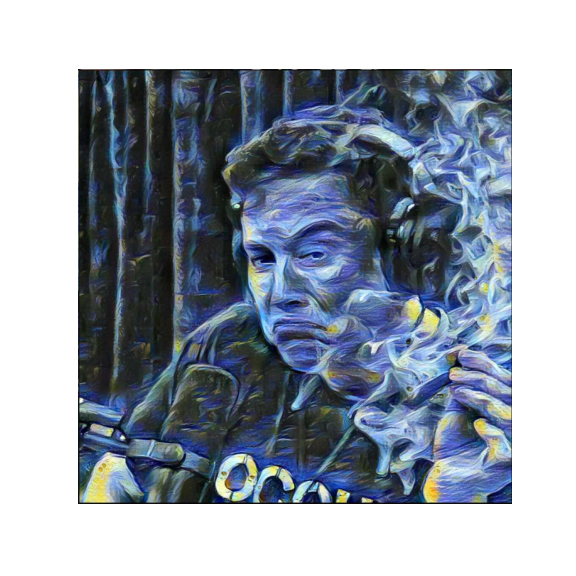
\includegraphics[scale=0.38]{assets/elon_canaGAN.png}
    \vspace{-50pt}
    \caption{Elon Musk}
  \end{minipage}
  \hfill
  \begin{minipage}[c]{0.49\linewidth}
    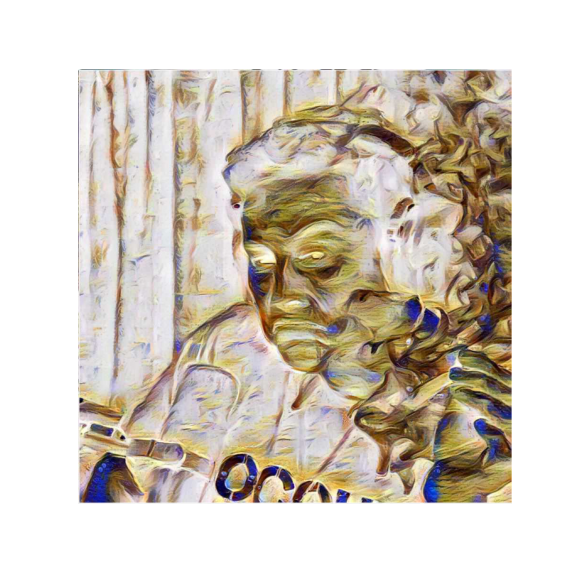
\includegraphics[scale=0.38]{assets/elon_inverted.png}
    \vspace{-50pt}
    \caption{Inverted filter}
  \end{minipage}
  \vspace{-20pt}
  \begin{minipage}[l]{0.49\linewidth}
    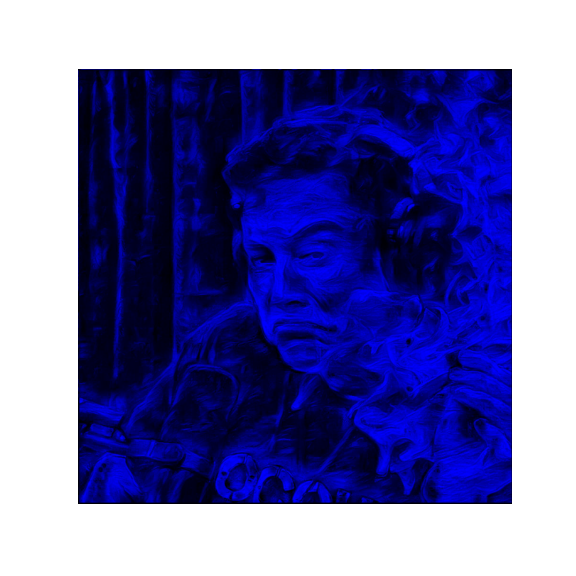
\includegraphics[scale=0.38]{assets/elon_blue.png}
    \vspace{-50pt}
    \caption{Blue filter}
  \end{minipage}
  \hfill
  \begin{minipage}[c]{0.49\linewidth}
    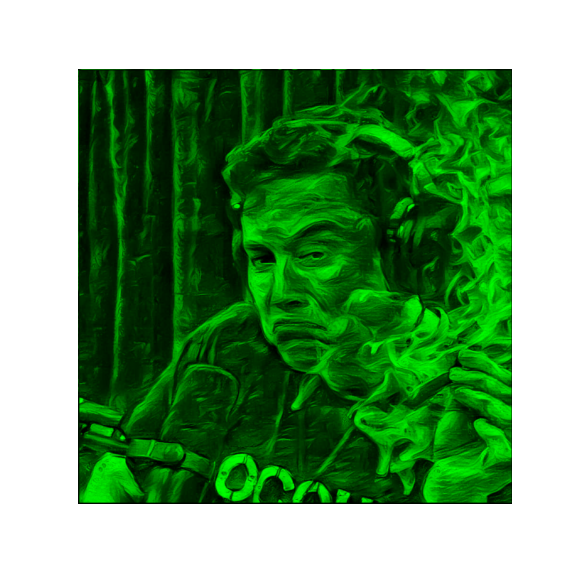
\includegraphics[scale=0.38]{assets/elon_green.png}
    \vspace{-50pt}
    \caption{Green filter}
  \end{minipage}
  \vspace{-20pt}
  \begin{minipage}[l]{0.49\linewidth}
    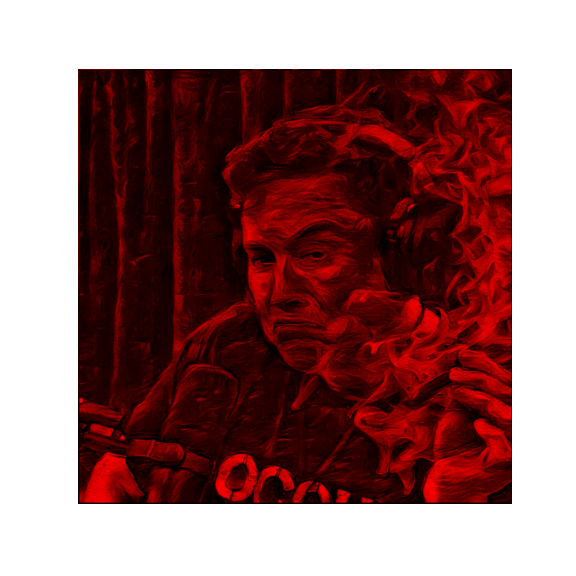
\includegraphics[scale=0.38]{assets/elon_red.png}
    \vspace{-50pt}
    \caption{Red filter}
  \end{minipage}
  \hfill
  \begin{minipage}[c]{0.49\linewidth}
    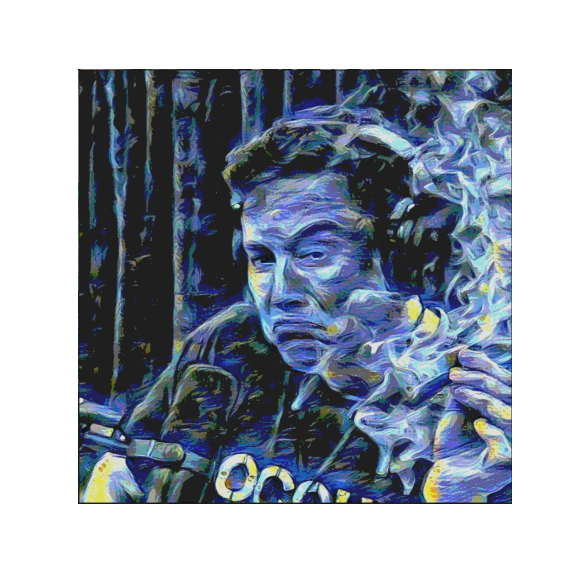
\includegraphics[scale=0.38]{assets/elon_celluloid.png}
    \vspace{-50pt}
    \caption{Celluloid filter}
  \end{minipage}
  
\end{figure}

\info{
The first image is a stylisation of elon musk that has been generated using a style transfer algorithm implemented in our lab.
You can see the code in 42AI repository \href{https://github.com/42-AI/StyleTransferMirror}{StyleTransferMirror}}

% ===========================(fin ex 03)         %
% ============================================== %

\newpage

% ============================================== %
% ===========================(start ex 04)       %
\chapter{Exercise 04}
\extitle{K-means Clustering}
\turnindir{ex04}
\exnumber{04}
\exfiles{Kmeans.py}
\exforbidden{Any functions allowing you to perform K-Means}
\makeheaderfilesforbidden

ALERT! DATA CORRUPTED

% ================================= %
\section*{Objective}
% --------------------------------- %
Implementation of a basic Kmeans algorithm.

% ================================= %
\section*{Instructions}
% --------------------------------- %
The solar system census dataset is corrupted! The citizens' homelands are missing!  
You must implement the K-means clustering algorithm in order to recover the citizens' origins.\\

You can find good explanations on how K-means is working here:
\href{https://bigdata-madesimple.com/possibly-the-simplest-way-to-explain-k-means-algorithm/}{Possibly the simplest way to explain K-Means algorithm}

The missing part is how to compute the distance between 2 data points (cluster centroid or a row in the data).
In our case the data we have to process is composed of 3 values (height, weight and bone\_density).
Thus, each data point is a vector of 3 values.
Now that we have mathematically defined our data points (vector of 3 values),
it is very easy to compute the distance between two points using vector properties.\\
You can use L1 distance, L2 distance, cosine similarity, and so forth...
Choosing the distance to use is called hyperparameter tuning.
I would suggest you to try with the easiest setting (L1 distance) first.\\

What you will notice is that the final result of the "training"/"fitting" will depend a lot on the random initialization.
Commonly, in machine-learning libraries, K-means is run multiple times
(with different random initializations) and the best result is saved.  


NB: To implement the fit function, keep in mind that a centroid can be considered as the gravity center of a set of points.  

Your program \texttt{Kmeans.py} takes 3 parameters: \texttt{filepath}, \texttt{max\_iter} and \texttt{ncentroid}:

\begin{42console}
  python Kmeans.py filepath='../ressources/solar_system_census.csv' ncentroid=4 max_iter=30
\end{42console}


it is expected by running your program to:
\begin{itemize}
  \item parse the arguments,
  \item read the dataset,
  \item fit the dataset,
  \item display the coordinates of the different centroids and the associated region (for the case \texttt{ncentroid=4}),
  \item display the number of individuals associated to each centroid,
  \item (Optional) display on 3 differents plots, corresponding to 3 combinaisons of 2 parameters,
    the results. Use different colors to distinguish  between Venus, Earth, Mars and Belt asteroids citizens.
\end{itemize}

Create the class \texttt{KmeansClustering} with the following methods:  

\begin{minted}[bgcolor=darcula-back,formatcom=\color{lightgrey},fontsize=\scriptsize]{python}
class KmeansClustering:
    def __init__(self, max_iter=20, ncentroid=5):
        self.ncentroid = ncentroid # number of centroids
        self.max_iter = max_iter # number of max iterations to update the centroids
        self.centroids = [] # values of the centroids
        
    def fit(self, X):
        """
        Run the K-means clustering algorithm.
        For the location of the initial centroids, random pick ncentroids from the dataset.
        Args:
        -----
          X: has to be an numpy.ndarray, a matrice of dimension m * n.
        Return:
        -------
          None.
        Raises:
        -------
          This function should not raise any Exception.
        """
        ... your code ...

    def predict(self, X):
        """
        Predict from wich cluster each datapoint belongs to.
        Args:
        -----
          X: has to be an numpy.ndarray, a matrice of dimension m * n.
        Return:
        -------
          the prediction has a numpy.ndarray, a vector of dimension m * 1.
        Raises:
        -------
          This function should not raise any Exception.
        """
        ... your code ...
\end{minted}

% ================================= %
\section*{Dataset}
% --------------------------------- %
The dataset, named \textbf{solar\_system\_census} can be found in
the resources folder.  
It is a part of the solar system census dataset, and contains biometric
informations such as the height, weight, and bone density of solar
system citizens.  

Solar citizens come from four registered areas:
\begin{itemize}
  \item The flying cities of Venus,
  \item United Nations of Earth,
  \item Mars Republic,
  \item Asteroids' Belt colonies.  
\end{itemize}

Unfortunately the data about the planets of origin was lost...  
Use your K-means algorithm to recover it!  
Once your clusters are found, try to find matches between clusters and the citizens' homelands.

\hint{
  \begin{itemize}
    \item People are slender on Venus than on Earth.  
    \item People of the Martian Republic are taller than on Earth.  
    \item Citizens of the Belt are the tallest of the solar system and have the lowest bone density due to the lack of gravity.  
  \end{itemize}
}

% ================================= %
\section*{Examples}
% --------------------------------- %
Here is an exemple of the algorithm K-means in action:\\
\url{https://i.ibb.co/bKFVVx2/ezgif-com-gif-maker.gif}


% ===========================(fin ex 04)         %
% ============================================== %

\newpage

% ================================= %
\section*{Contact}
% --------------------------------- %
You can contact 42AI association by email: contact@42ai.fr\\
You can join the association on \href{https://join.slack.com/t/42-ai/shared_invite/zt-ebccw5r7-YPkDM6xOiYRPjqJXkrKgcA}{42AI slack}
and/or posutale to \href{https://forms.gle/VAFuREWaLmaqZw2D8}{one of the association teams}.

% ================================= %
\section*{Acknowledgements}
% --------------------------------- %
The modules Python \& ML is the result of a collective work, we would like to thanks:
\begin{itemize}
  \item Maxime Choulika (cmaxime),
  \item Pierre Peigné (ppeigne, pierre@42ai.fr),
  \item Matthieu David (mdavid, matthieu@42ai.fr),
  \item Quentin Feuillade--Montixi (qfeuilla, quentin@42ai.fr)
\end{itemize}
who supervised the creation, the enhancement and this present transcription.

\begin{itemize}
    \item Louis Develle (ldevelle, louis@42ai.fr)
    \item Augustin Lopez (aulopez)
    \item Luc Lenotre (llenotre)
    \item Owen Roberts (oroberts)
    \item Thomas Flahault (thflahau)
    \item Amric Trudel (amric@42ai.fr)
    \item Baptiste Lefeuvre (blefeuvr@student.42.fr)
    \item Mathilde Boivin (mboivin@student.42.fr)
    \item Tristan Duquesne (tduquesn@student.42.fr)
\end{itemize}
for your investment for the creation and development of these modules.

\begin{itemize}
    \item Barthélémy Leveque (bleveque@student.42.fr)
    \item Remy Oster (roster@student.42.fr)
    \item Quentin Bragard (qbragard@student.42.fr)
    \item Marie Dufourq (madufour@student.42.fr)
    \item Adrien Vardon (advardon@student.42.fr)
\end{itemize}
who betatest the first version of the modules of Machine Learning.
\vfill
\doclicenseThis

\end{document}